\stopallthesefloats{}
\subsection{Modeling Shared Buses}
\begin{figure}[hbt!]
\begin{center}
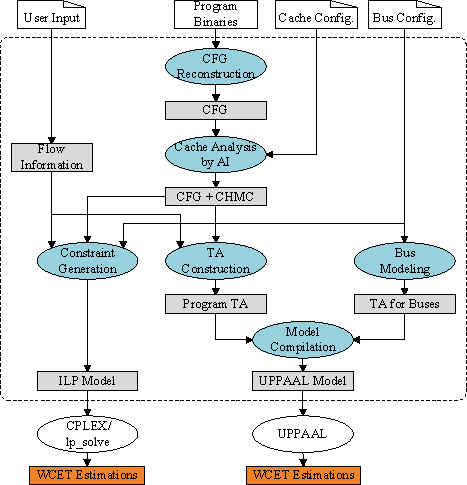
\includegraphics[width=0.7\textwidth]{\chapterdirectory/figure/analysis/mingsong.pdf}
\end{center}
\caption{Overall strategy for \cite{5702243} (taken from the paper)}%
\label{fig:formal_analysis:mingsong}
\end{figure}

The approach proposed by \cite{5702243} combines abstract interpretation and
model checking to compute WCET in multicore, with a special focus on the
interconnect. The abstract interpretation is found in the analysis of the
caches, which is done in a fashion similar to those presented in
Section~\ref{sec:rel_work:handling_it:accepting_it}, including in its remarks
of a previous approach being unsafe and in its omission of data caches (and
thus, of cache coherence). The overall strategy for this approach is shown in
Figure~\ref{fig:formal_analysis:mingsong}.

\begin{figure}[hbt!]
\begin{center}
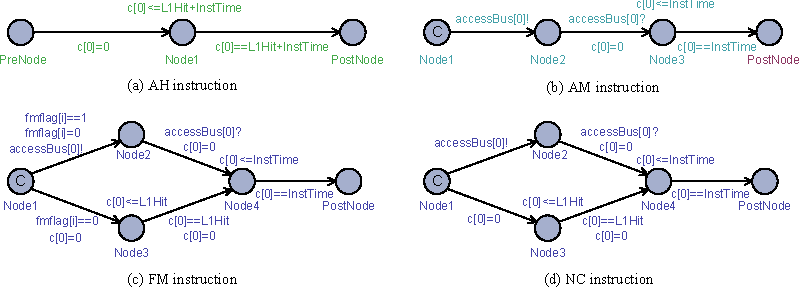
\includegraphics[width=\textwidth]{\chapterdirectory/figure/analysis/mingsong_program_block.pdf}
\end{center}
\caption{Program Model Building Blocks (taken from \cite{5702243})}%
\label{fig:formal_analysis:mingsong_prog_blocks}
\end{figure}

\begin{figure}[hbt!]
\begin{center}
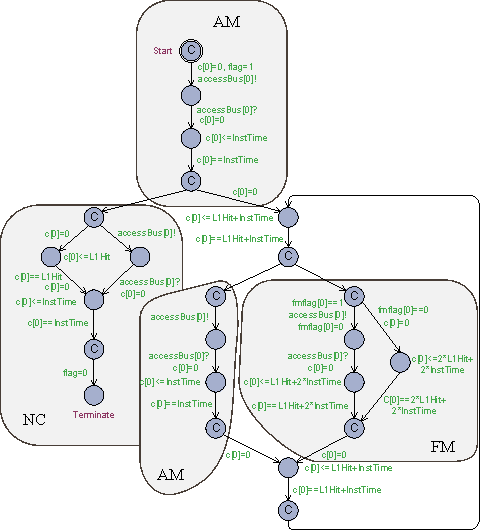
\includegraphics[width=\textwidth]{\chapterdirectory/figure/analysis/mingsong_program.pdf}
\end{center}
\caption{Program Example (adapted from \cite{5702243})}%
\label{fig:formal_analysis:mingsong_program}
\end{figure}

The resulting model considers program instructions only as their categorization
(\textit{Always Hits}, \textit{Always Misses}, \textit{First time Misses},
\textit{Not Categorized}). The paper proposes an automaton for each category
(see Figure~\ref{fig:formal_analysis:mingsong_prog_blocks}),
indicating how an instruction of this category will use the
interconnect. Models for program are thus constructed by replacing each
instruction in the control flow graph by the automaton corresponding to its
synchronization with the interconnect
(\textit{TA Construction} in Figure~\ref{fig:formal_analysis:mingsong}). An
example of resulting automaton can be seen in
Figure~\ref{fig:formal_analysis:mingsong_program}.

To showcase how modular the approach is in its modeling of the interconnect,
\cite{5702243} provides both a model for a TDMA bus and for a FCFS
(\textit{First Come, First Served}, which means requests are completed in the
order of their arrival) bus.

Figure~\ref{fig:formal_analysis:mingsong} mentions an ILP model being computed
as well, however, the paper does not make any mention of it.

\stopallthesefloats{}
